\documentclass[a4paper]{article}
\usepackage[utf8]{inputenc}

\usepackage{minted}
\usepackage{listings}

\usepackage{graphicx}
\usepackage{geometry}
 \geometry{
 a4paper,
 total={170mm,257mm},
 left=30mm,
 right=30mm,
 top=20mm,
 }
\title{Wireless networking project}
\author{
    Joseph Verburg (4018575, j.p.verburg@student.tudelft.nl)
}
\date{April 2018}

\begin{document}

\maketitle

\section{Introduction}
In this project we review and attempt to improve the rate control algorithm for 802.11ac standard to maximize throughput and thus minimize error rate.
\section{Method}
The method we use to approach this project is divided in 3 steps which we will elaborate on below.

\subsection{Understand behaviour of different modulation techniques}
The 802.11ac standard supports 3 modulation techniques: BPSK, QPSK and QAM which are divided into 10 levels based on modulation level and/or forward error correction ratio. Furthermore 4 different bandwidth levels are supported: 20, 40, 80 and 160 MHz. To properly understand how every modulation technique performs we simulate different snr levels for every bandwidth and modulation level.
\subsection{Establish basic algorithm}
From the simulation from the previous step we establish a look up table for every bandwidth and modulation level between which SNR levels it should be used.
We compare the performance for this algorithm to the base algorithm and tweak the the edges of different modulation levels to improve the stability where possible. It is expected that this will not be perfect because the algorithm will lag behind the behaviour of the channel.
\subsection{Extend the basic algorithm}
Using an history window we try to predict the expected SNR of the next packet to more accurately modulate and improve throughput.

\section{Simulation of different modulation techniques}
\begin{figure}[h]
\centering
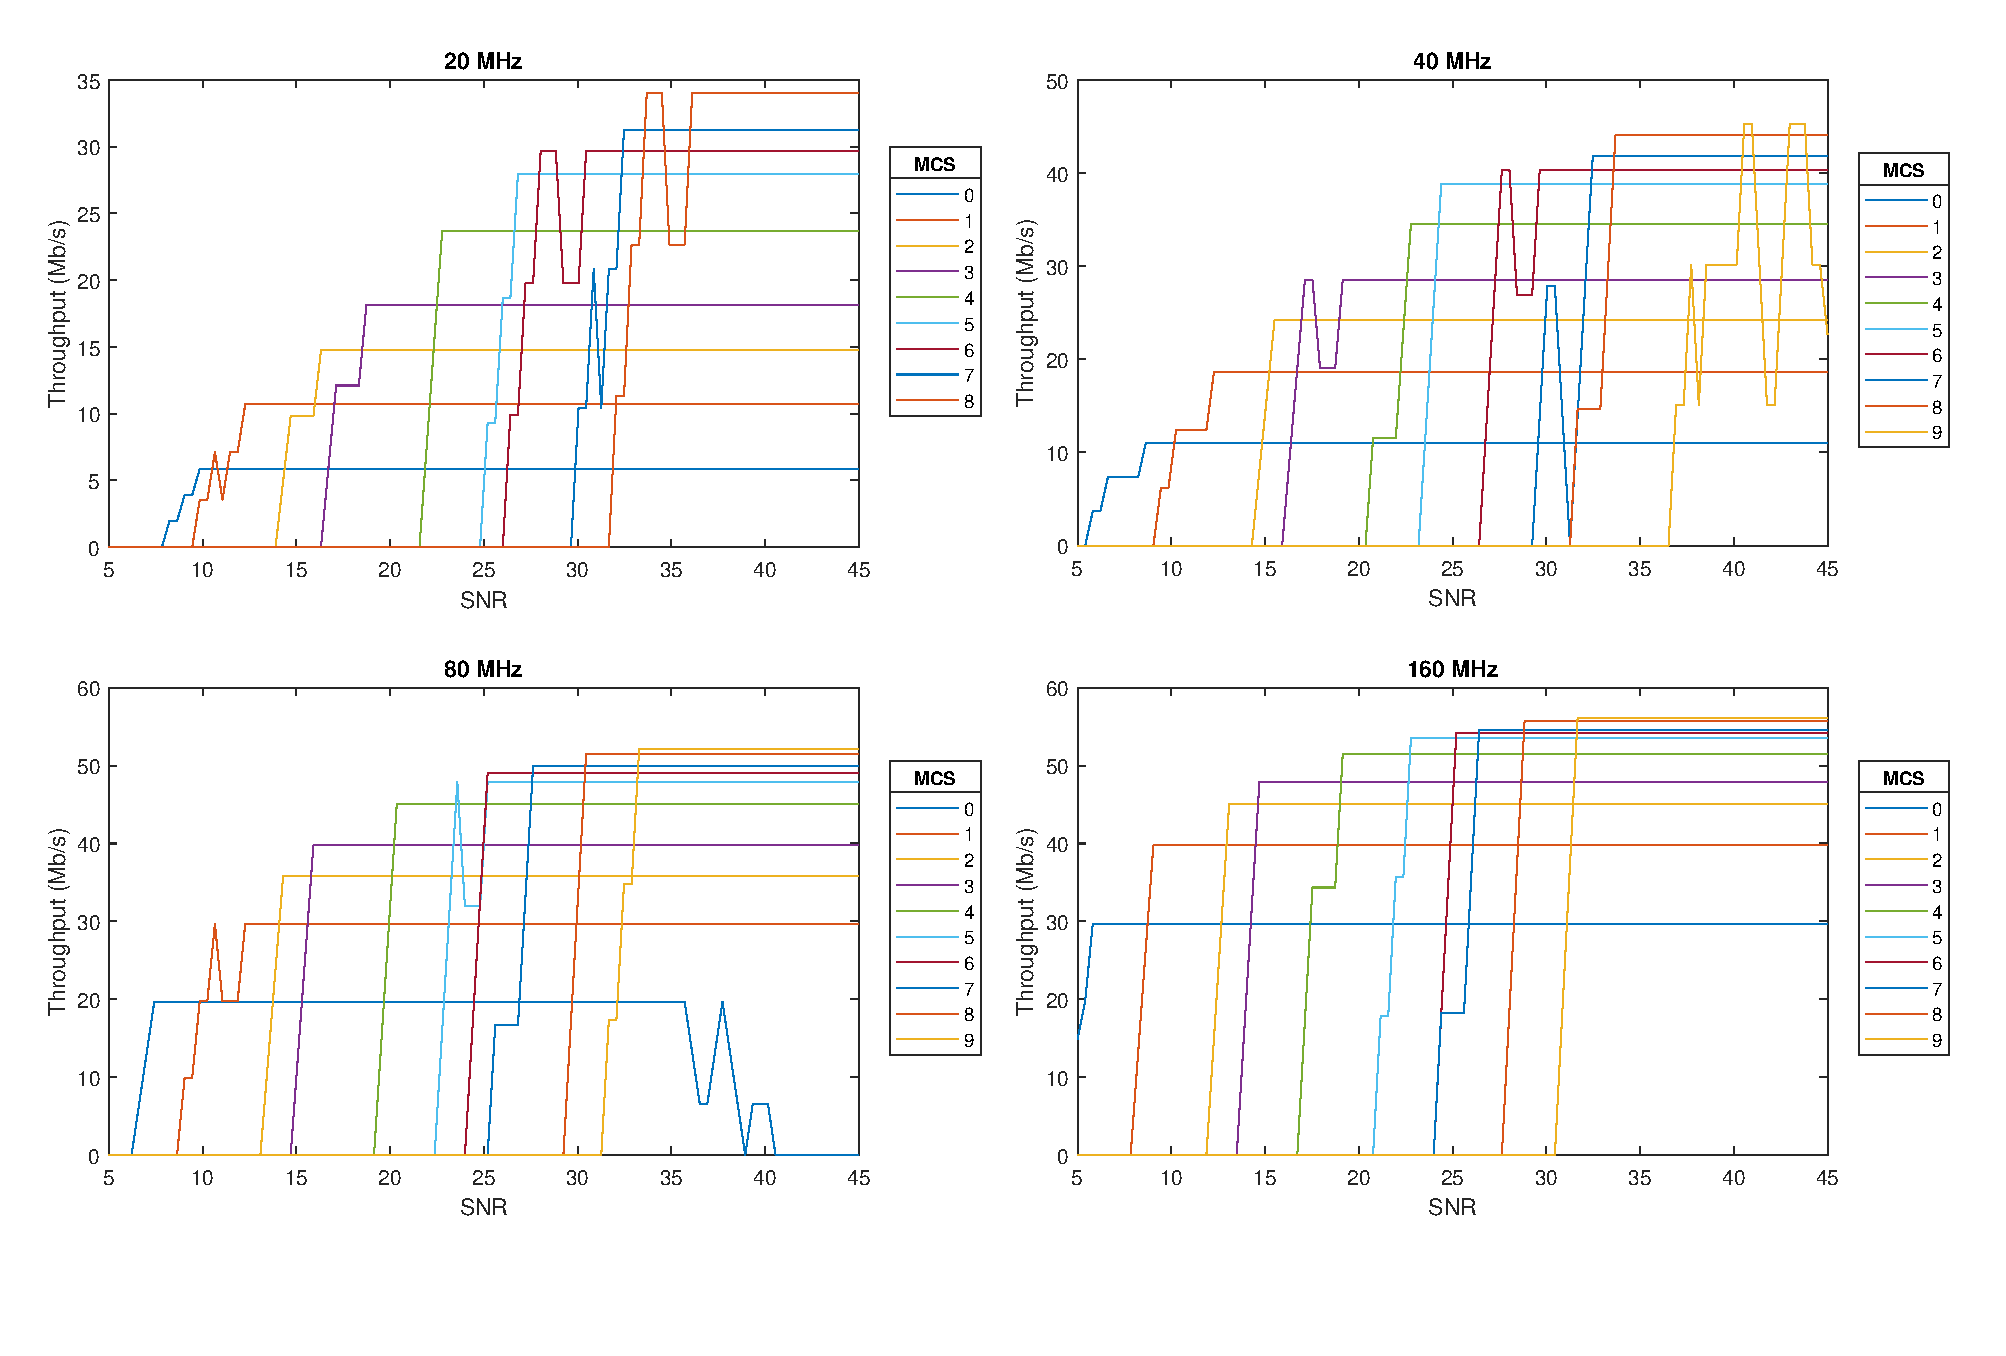
\includegraphics[scale=0.5]{steponev2.eps}
\caption{Different bandwidth and MCS combinations compared based on SNR and throughput. Every subplot is a different bandwidth.}
\label{fig:stepone}
\end{figure}
 The simulation results can be seen in Figure \ref{fig:stepone}. These results are achieved by taking the mean over 10 runs per bandwidth and MCS combination to get reliable results. From these results we concluded the following properties:
 \begin{itemize}
     \item Modulation level 0 is a good starting point when no previous channel information exists.
     \item For 20 MHz bandwidth level 9 is not supported. From the level 9 simulation of the 40 MHz bandwidth we see why, this modulation level does not perform well under low bandwidth. After some research we find that the level 9 is explicitly not added for the 20 MHz bandwidth by the 802.11ac standard.
     \item Like previously mentioned, level 9 performs very bad under 40 MHz bandwidth and thus should be avoided.
     \item For 80 MHz bandwidth level 5 does not offer improvements compared to higher levels and should be avoided. This can be somewhat explained by the fact that level 5 and 6 have the same modulation technique namely 64QAM and only $11\%$ difference in coding scheme redundancy. We conclude that this extra redundancy of level 5 does not help under this bandwidth to improve reliability.
     \item For 80 and 160 MHz bandwidth level 9 does perform well and can be used.
 \end{itemize}
 Furthermore we established the SNR lookup table for every bandwidth from these simulations. Where the SNR is used from the first value where the modulation level stabilizes.
 
\section{Testing basic algorithm}

\begin{figure}[h]
\centering
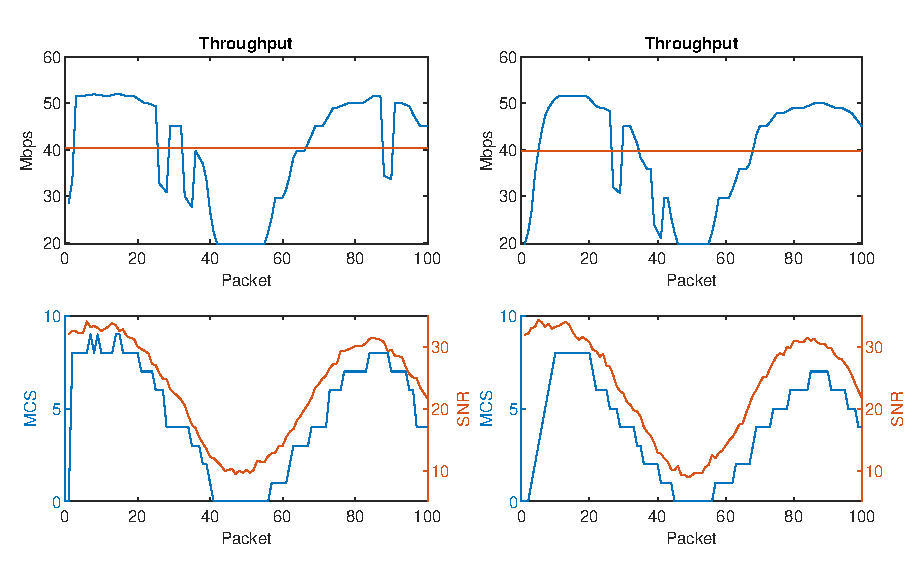
\includegraphics[scale=1]{steptwo80.eps}
\caption{Basic algorithm (left) and original algorithm (right) compared at 80MHz bandwidth. Average throughput displayed as horizontal line.}
\label{fig:steptwo_single}
\end{figure}
First we tuned the algorithm by testing the algorithm for every bandwidth and seeing where the edges were too tight or too loose. 
During this tuning we also found that the already excluded modulation for the 20 and 40 MHz bandwidth is also sensitive under higher bandwidths and thus for stable operation we increased the minimum SNR for that level in the algorithm beyond what we established in the simulation.\\
One simulation of the tuning can be seen in Figure \ref{fig:steptwo_single} where we compare it to original algorithm. We already see that the algorithm performs better then the original in average throughput. Furthermore the expected lagging can also be seen by the various sudden dips where the algorithms does not choose the best MCS because it does not know that the channel is deteriorating.\\
\begin{figure}[h!]
\centering
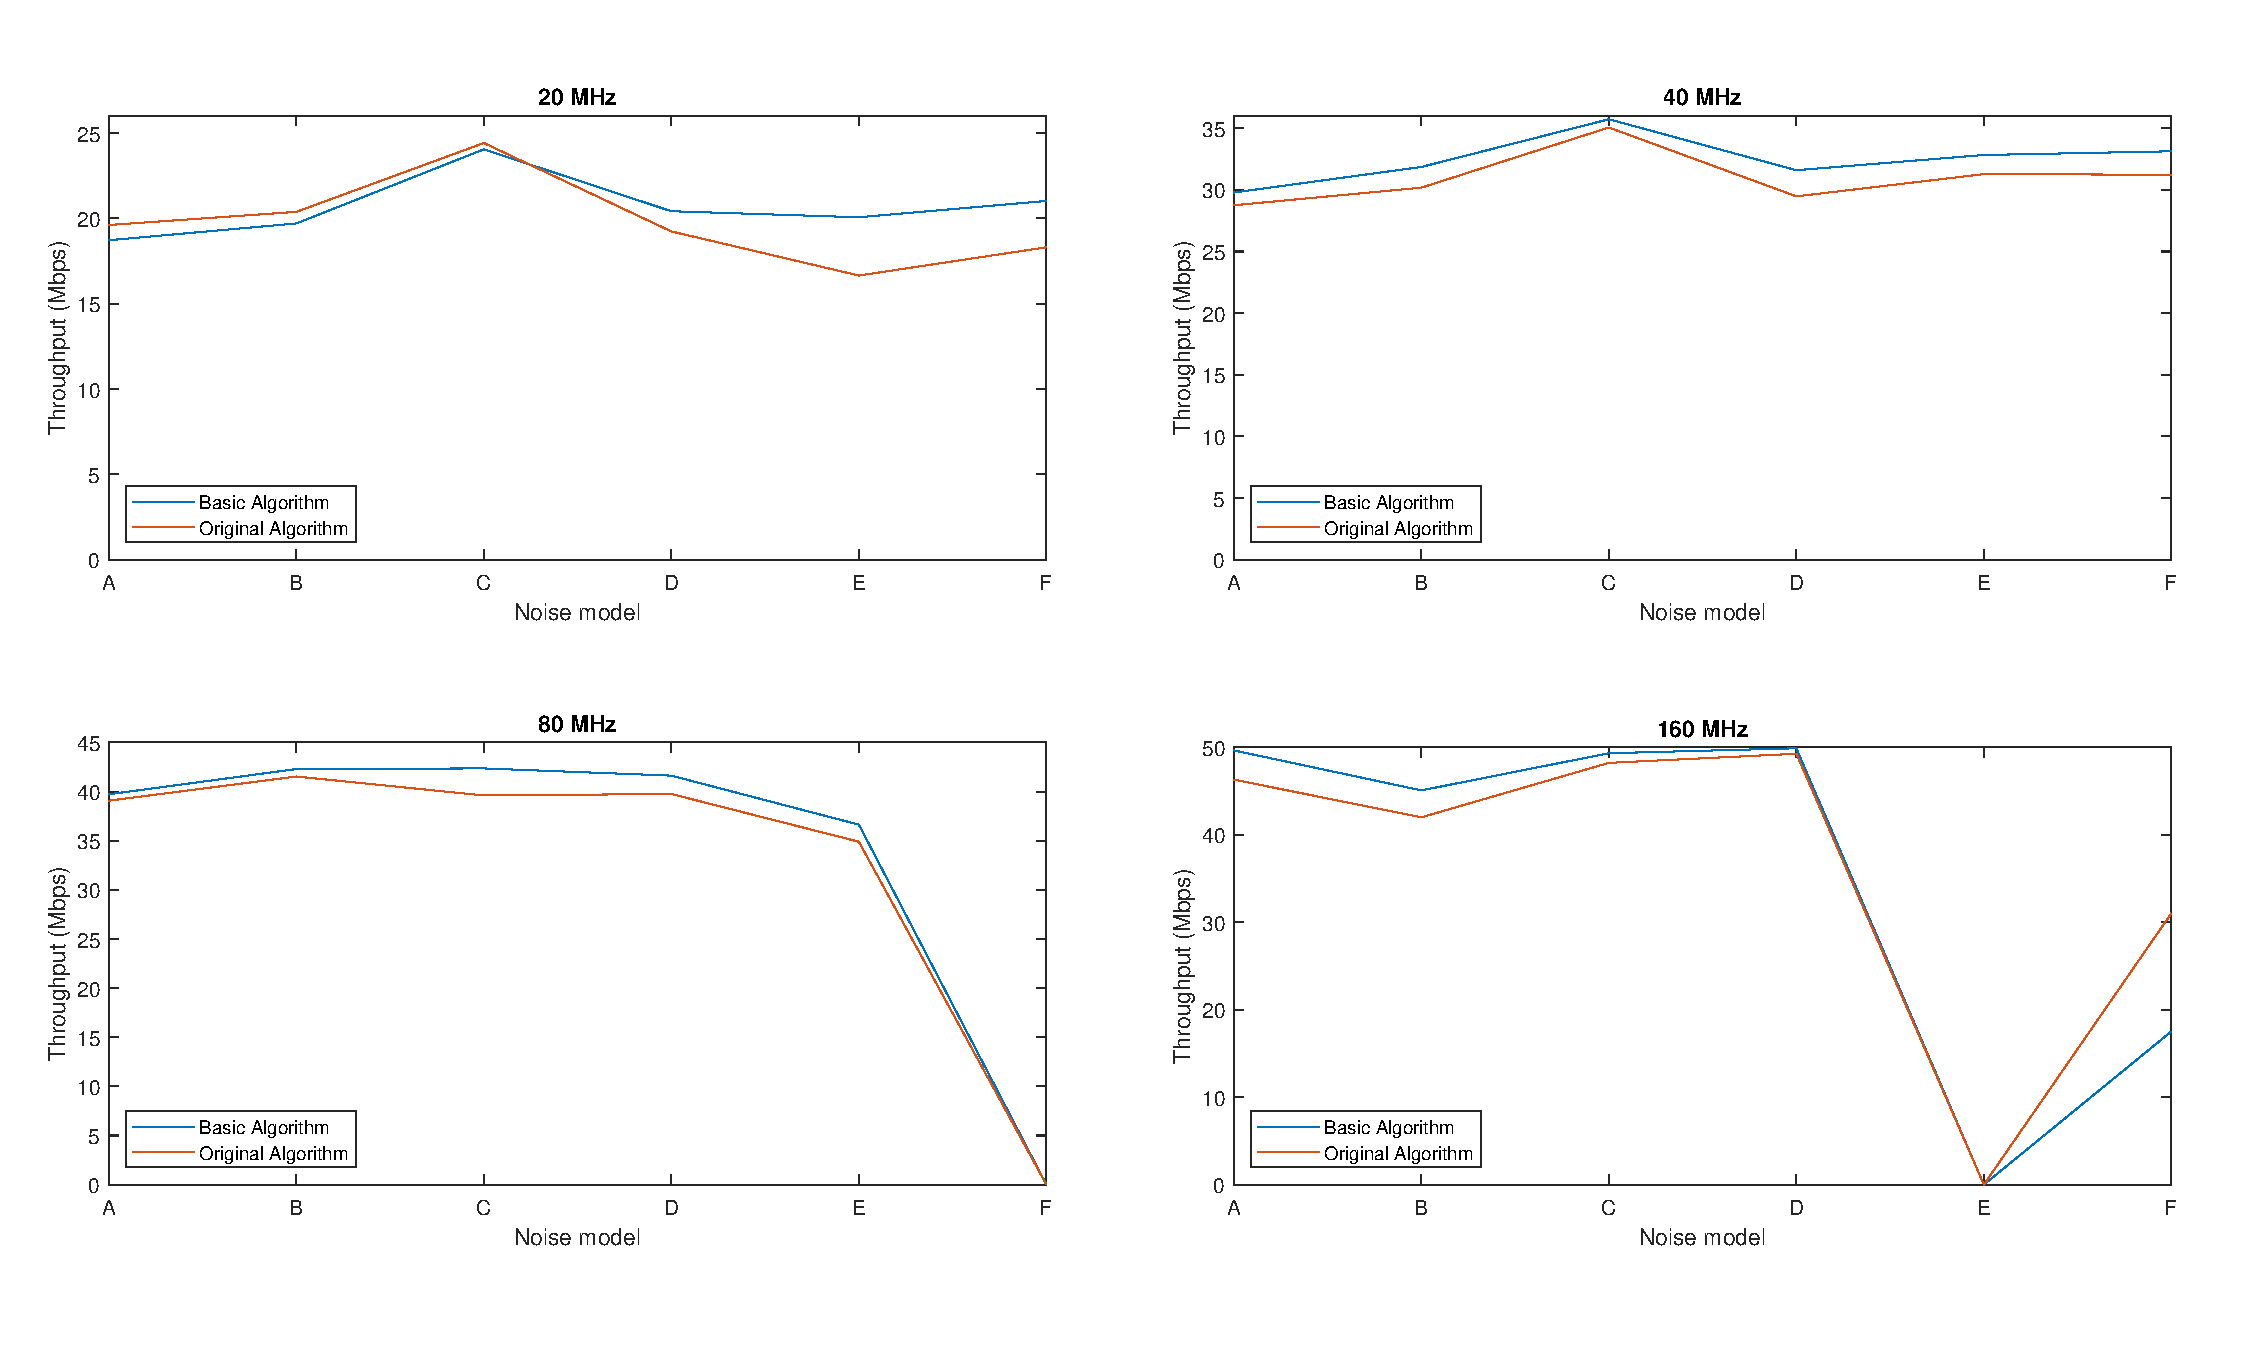
\includegraphics[scale=.4]{steptwo.eps}
\caption{Comparison of the 2 algorithms under various noise models and bandwidths.}
\label{fig:steptwo}
\end{figure}
The complete comparison under all bandwidths can be seen in Figure \ref{fig:steptwo}. We see that an clear improvement in throughput is achieved by using our algorithm. Furthermore we see that the simulation does not work properly for Model F under 80 MHz and Model E and F under 160 MHz, thus these will be ignored in the next simulation. On average an increase of 1.44 Mbps is achieved, which is considerable as the original algorithm already performs very well.
\clearpage
\section{Testing extended algorithm}
\begin{figure}[h!]
\centering
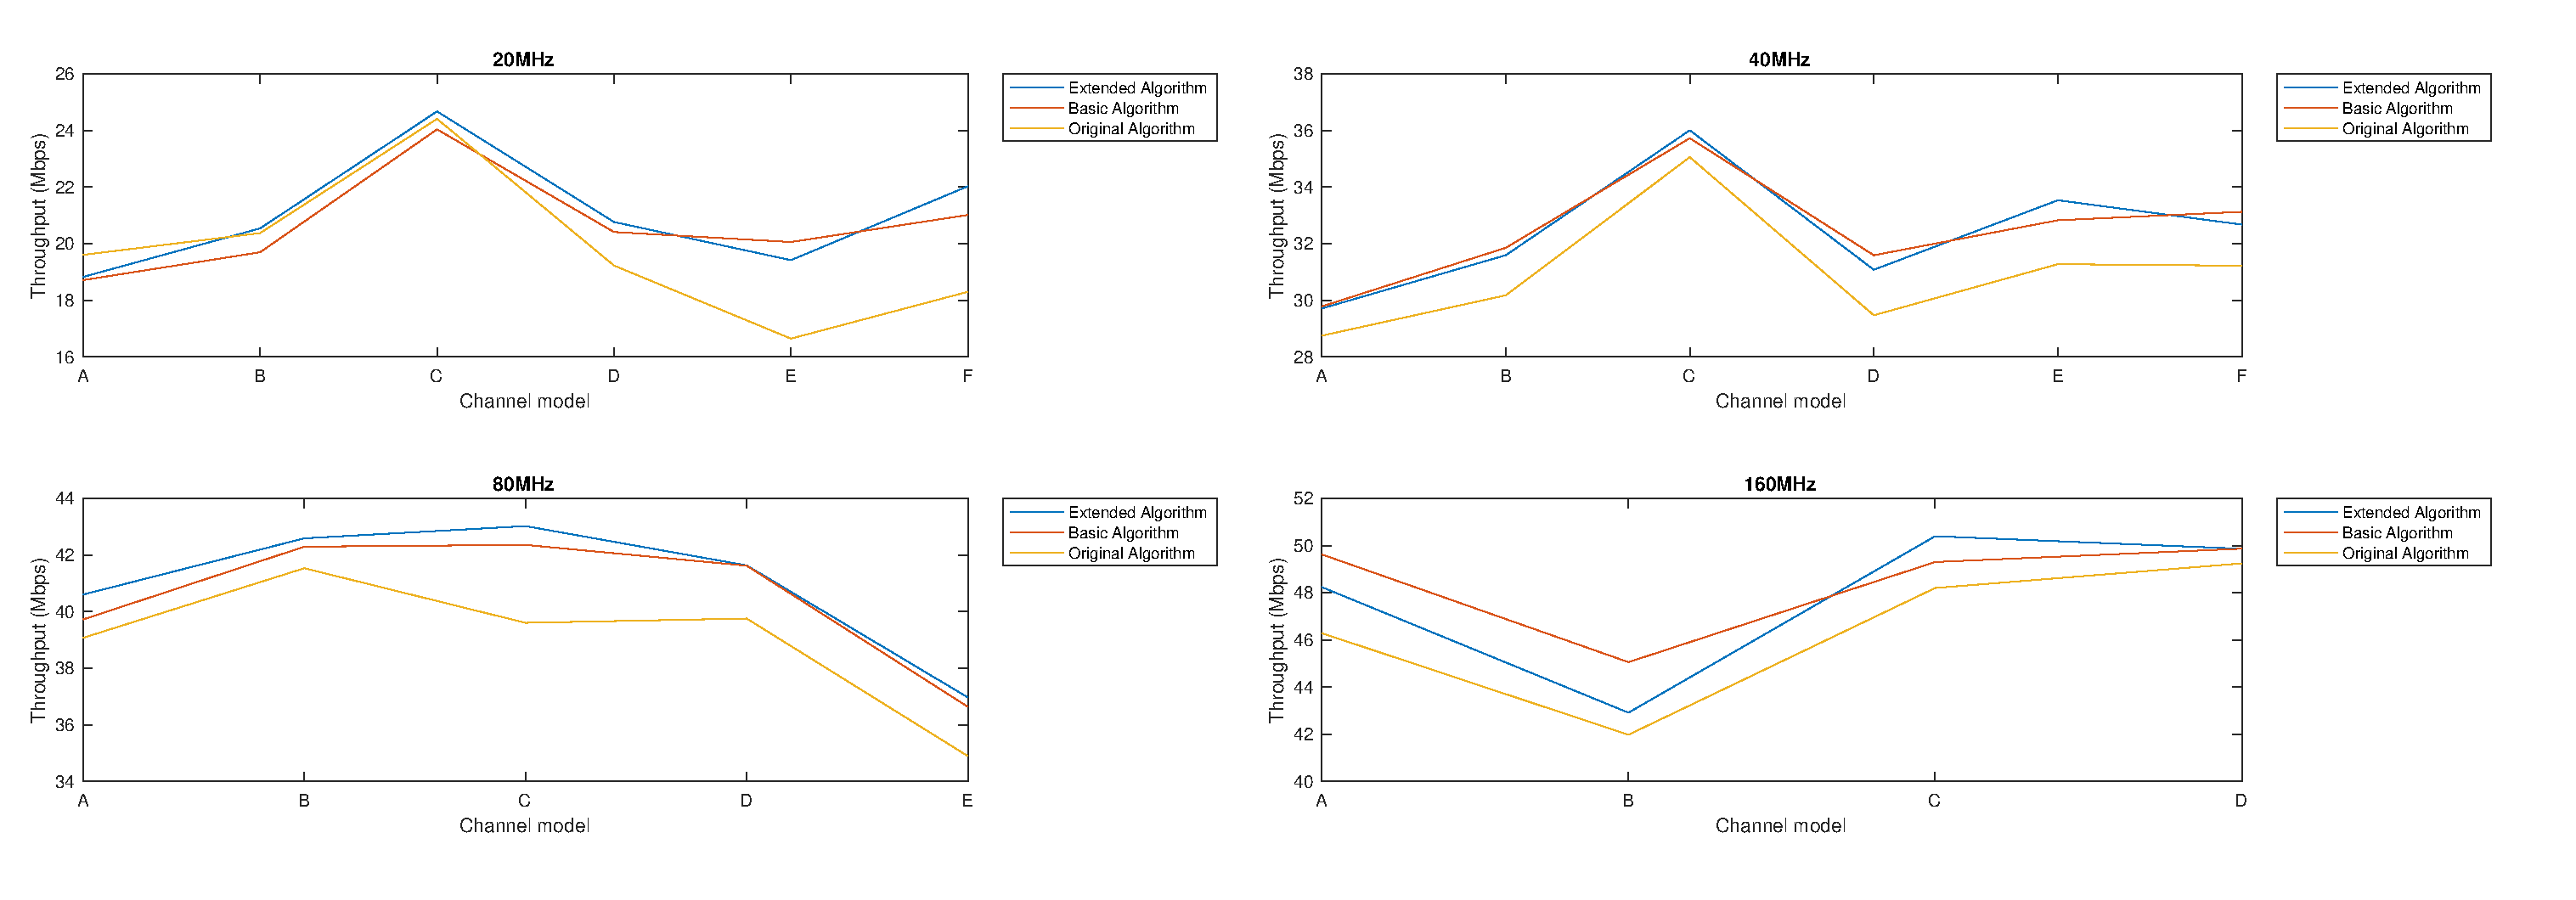
\includegraphics[scale=.35]{stepthree.eps}
\caption{Comparison of the 3 algorithms under various noise models and bandwidths.}
\label{fig:stepthree}
\end{figure}
For the extended algorithm we used the same lookup tables established for the basic algorithm and extend the algorithm with predictive behaviour to more accurately predict the SNR of the next packet in a changing environment. The prediction works by using the SNR values of previously received packets and finding a trend in these values. In the initial start of the algorithm we fallback to the method of the basic algorithm until we have enough historic SNR values.\\
We used a polynomial fit function to detect the trend. We experimented with first and second order polynomial fit where we found that the second order outperformed the first order polynomial fit. We also experimented with different sizes of history length used in the polynomial fit, where a history size of 5 worked best.\\
The performance the extended algorithm can be seen in Figure \ref{fig:stepthree}. As already noted there are several model bandwidth combinations that don't work thus these have been removed from the results.
From the results we see that the extended algorithm is an improvement over the basic algorithm. There are a few situations where the extended algorithm under-performs, but this can be explained that the algorithm predicts to eagerly and thus lowers the modulation level prematurely. Compared to the original algorithm the extended algorithm on average performs 1.52 Mbps better compared to the 1.44 Mbps increase of the basic algorithm. A possible explanation for the smaller increase is that there was ample space to improve from the original algorithm but that the basic algorithm already covered most of it and thus only minor space is left to improve upon. A second explanation is as we already noted the too eager prediction of the algorithm where it too early or too late switches modulation level. 
\section{Conclusion}
Our proposed method and algorithm achieved an improvement compared to the original algorithm. What is especially interesting to note is that the biggest improvements are in more difficult channel models which results in a more stable communication which is desirable. Furthermore the proposed basic algorithm is implementation wise simpler then the original algorithm while increasing the performance and reliability. What was also noticed during simulation is that the current channel models are far from perfect when using the higher bandwidths functioning barely or not at all. During simulation it was also noticed that the 2 higher bandwidths (80 and 160 MHz) had ample headroom left under higher SNR values (especially under the 160 MHz bandwidth) which indicates that higher QAM modulation levels are possible. After some research online we found that this is already done by some manufacturers that support the non standard 1024QAM modulation which further increases the throughput under the higher bandwidths.
\end{document}
